\documentclass[]{beamer}
\usepackage{amsmath, amssymb}
\usepackage{graphicx}
\usepackage{colortbl}
\usepackage{arydshln}
\usepackage{color}

\usepackage{setspace}			% Allows for local line spacing control (eg \setstretch)
\usepackage[comma]{natbib} 		% For author-year citations
\usepackage{tikz} 				% Used for backgrounds (and also for diagrams)
\setbeamertemplate{navigation symbols}{} % Supresses navigation symbols that would appear at bottom
\setbeamertemplate{enumerate items}[circle] % Changes beamers bullets to circle
\setbeamertemplate{itemize items}[circle] % Changes beamers bullets to circle

%%%%%%%%%%%%%%%%%%%%%%%%%%%%%%%%%%%%%%%%%%%%%%%%%%%%%%%%%%%%%%%%%%%%%%%%%%%%%%%%%
% Allows For Tikz Image Placement (Among other things)
%%%%%%%%%%%%%%%%%%%%%%%%%%%%%%%%%%%%%%%%%%%%%%%%%%%%%%%%%%%%%%%%%%%%%%%%%%%%%%%%%
\usepackage{tikz} 				% Used for backgrounds (and also for diagrams)
\usetikzlibrary{overlay-beamer-styles}
\tikzset{
	use page relative coordinates/.style={
		shift={(current page.south west)},
		x={(current page.south east)},
		y={(current page.north west)}
	},
}
\usetikzlibrary {shapes.geometric}		% Allows more shapes for nodes

%%%%%%%%%%%%%%%%%%%%%%%%%%%%%%%%%%%%%%%%%%%%%%%%%%%%%%%%%%%%%%%%%%%%%%%%%%%%%%%%%
% Commands for Light vs Dark Backgrounds
%%%%%%%%%%%%%%%%%%%%%%%%%%%%%%%%%%%%%%%%%%%%%%%%%%%%%%%%%%%%%%%%%%%%%%%%%%%%%%%%%
% Call the command right before the slide (outside of the frame envinronmet). The
%    chosen background will persist until the other command is called.

\newcommand{\UseLightBackground}{
	\usebackgroundtemplate{
		\tikz[overlay,remember picture] \node[opacity=1.6, at=(current page.center)] 
		{ 
\includegraphics[height=\paperheight,width=\paperwidth]{img/Background_Light_Blank.png} };
	}
}
\newcommand{\UseDarkBackground}{
	\usebackgroundtemplate{
		\tikz[overlay,remember picture] \node[opacity=1.6, at=(current page.center)] 
		{ 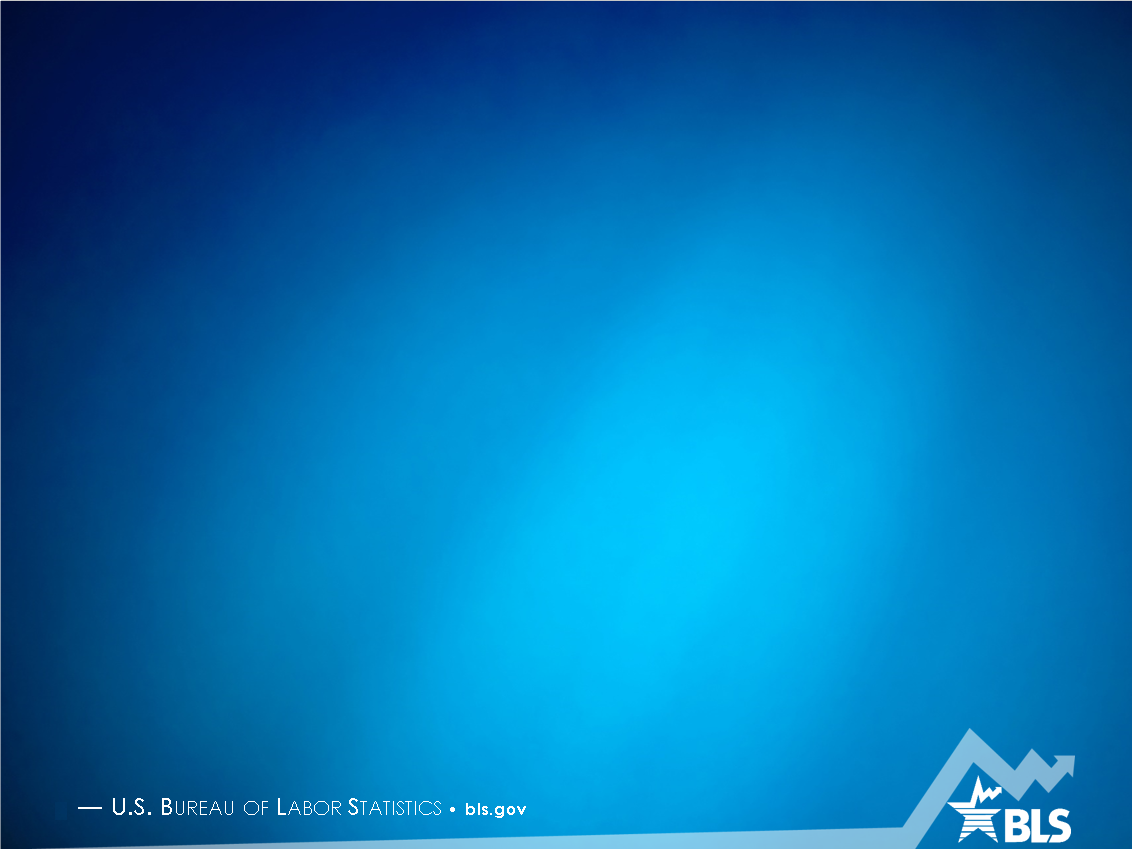
\includegraphics[height=\paperheight,width=\paperwidth]{img/Background_Dark.png} };
	}
}

%%%%%%%%%%%%%%%%%%%%%%%%%%%%%%%%%%%%%%%%%%%%%%%%%%%%%%%%%%%%%%%%%%%%%%%%%%%%%%%%%
% Creates Section Signposts
%%%%%%%%%%%%%%%%%%%%%%%%%%%%%%%%%%%%%%%%%%%%%%%%%%%%%%%%%%%%%%%%%%%%%%%%%%%%%%%%%
%%%%% Can disable for a section using "\NextSectionWithoutTitlePage"

\newif\ifSectionTitlePage
\newcommand\NextSectionWithoutTitlePage{\SectionTitlePagefalse}
\SectionTitlePagefalse			% Turning off the TOC slides
\AtBeginSection[]
{
	\ifSectionTitlePage
%	\UseLightBackground  % Use the BLS background
%	\setbeamertemplate{footline}[reg page number]
	\begin{frame}
		\frametitle{Presentation Outline}
		\tableofcontents[currentsection]
	\end{frame}
	\fi
	\SectionTitlePagetrue % Turns section pages on for subsequent
}
\AtBeginSubsection[]
{
	\begin{frame}
		\frametitle{Table of Contents}
		\tableofcontents[currentsection,currentsubsection]
	\end{frame}
}

%%%%%%%%%%%%%%%%%%%%%%%%%%%%%%%%%%%%%%%%%%%%%%%%%%%%%%%%%%%%%%%%%%%%%%%%%%%%%%%%%
% Defining BLS Colors and Slide Number Footnotes
%%%%%%%%%%%%%%%%%%%%%%%%%%%%%%%%%%%%%%%%%%%%%%%%%%%%%%%%%%%%%%%%%%%%%%%%%%%%%%%%%
\definecolor{mygray}{gray}{0.30} % Defining gray color for footnotes
\definecolor{navyblue}{rgb}{0.0, 0.0, 0.5}
\defbeamertemplate{footline}{left page number}
{%
  \hfill%
  \usebeamercolor[white]{page number in head/foot}%
  \usebeamerfont{page number in head/foot}%
  %  \insertframenumber\,/\,\inserttotalframenumber \ -- U.S. Bureau of Labor Statistics \ -- bls.gov \kern33em
  \vskip10pt%
}
\setbeamertemplate{footline}[left page number]
\defbeamertemplate{footline}{reg page number}
{%
  \hfill%
  \usebeamercolor[navyblue]{page number in head/foot}%
  \usebeamerfont{page number in head/foot}%
  \insertframenumber\,/\,\inserttotalframenumber \ -- U.S. Bureau of Labor Statistics \ -- bls.gov \kern33em\vskip10pt%
}

%%%%%%%%%%%%%%%%%%%%%%%%%%%%%%%%%%%%%%%%%%%%%%%%%%%%%%%%%%%%%%%%%%%%%%%%%%%%%%%%%
% Main Presentation Slides 
%%%%%%%%%%%%%%%%%%%%%%%%%%%%%%%%%%%%%%%%%%%%%%%%%%%%%%%%%%%%%%%%%%%%%%%%%%%%%%%%%

\begin{document}
\title{\textbf{\textcolor{white}{TITLE: \\ SUBTITLE}}}
\author{\textbf{\textcolor{white}{Elan Segarra}} \\ \normalsize{\textcolor{white}{U.S. Bureau of Labor Statistics}}}
%\institute{\normalsize{\textcolor{white}{U.S. Bureau of Labor Statistics}}}
\date{\textcolor{white}{Conference/Seminar Name \\ \vspace{.05cm} Month DD, YYYY}}

\UseDarkBackground
\begin{frame}[noframenumbering]\textcolor{white}{
  \titlepage
  \vspace{-1em}\textcolor{white}{
  	{\setstretch{0.75}\scriptsize{Disclaimer: The views expressed herein are those of the author(s) and do not necessarily reflect those of the Federal Government, Department of Labor, or the Bureau of Labor Statistics.	All results have been reviewed to ensure that no confidential information is disclosed.\\}}
  }
}\end{frame}

\UseLightBackground
\setbeamertemplate{footline}[reg page number]
\begin{frame}{Motivations}
	\begin{enumerate}
		\item ...
		\item ...
	\end{enumerate}
\end{frame}

\begin{frame}{Presentation Overview}
	\begin{itemize}
		\item {\Large Part 1:}
			\begin{itemize}
				\item ...
				\item ...
			\end{itemize}
		\bigskip
		\item {\Large Part 2:}
			\begin{itemize}
				\item ...
				\item ...
			\end{itemize}
		\bigskip
		\item {\Large Part 2:}
		\begin{itemize}
			\item ...
			\item ...
		\end{itemize}
	\end{itemize}
\end{frame}

\UseDarkBackground
\begin{frame}[noframenumbering, plain]
	\textcolor{white}{
		\begin{center}
			{\LARGE  Part 1}
		\end{center}}
\end{frame}
\UseLightBackground

\begin{frame}{Something}
	
\end{frame}

\begin{frame}{Something Else}
	
\end{frame}

\begin{frame}{Summary}
	This is what was done:
	\begin{itemize}
		\item ...
		\item ...
	\end{itemize}
	
	\bigskip
	Future work:
	\begin{itemize}
		\item ...
		\item ...
	\end{itemize}
\end{frame}

%}

\UseDarkBackground
\setbeamertemplate{footline}[left page number]
\begin{frame}[noframenumbering]{\textcolor{white}{CONTACT INFORMATION}}
	\begin{center}
		\textcolor{white}{\huge{Thank You!}}
		\bigskip
		\bigskip
		
%		\textcolor{white}{\Large\textbf{Elan Segarra}}

		\textcolor{white}{\large U.S. Bureau of Labor Statistics \\ Office of Compensation and Working Conditions \\ \phantom{} \\ Segarra.Elan@BLS.gov}
	\end{center}

\end{frame}

%%%%%%%%%%%%%%%%%%%%%%%%%%%%%%%%%%%%%%%%%%%%%%%%%%%%%%%%%%%%%%%%%%%%%%%%%%%%%%%%%
% APPENDIX 
%%%%%%%%%%%%%%%%%%%%%%%%%%%%%%%%%%%%%%%%%%%%%%%%%%%%%%%%%%%%%%%%%%%%%%%%%%%%%%%%%

%\appendix
%\begin{frame}[allowframebreaks, noframenumbering]{Bibliography}
%	\bibliographystyle{apa}
%	\textcolor{white}{\bibliography{bib_file_name}}  % The bib file(s)
%\end{frame}
%
%\UseLightBackground
%\setbeamertemplate{footline}[left page number]
%
%\begin{frame}[label=extra_details]{Something Extra}
%	Something a little extra here, just in case more details are required (or more time needs to be killed)
%	
%	Back to \hyperlink{situation2}{\beamerbutton{main slide}}.
%\end{frame}

\end{document}